\chapter{向前走} \label{chap:chap13}


我们必须有意识地走完通往目标的路程的一部分,然后在黑暗中迈向成功。
\begin{flushright}
	——亨利$\cdot$戴维$\cdot$梭罗
\end{flushright}


\begin{figure}[!htb]
	\centering
	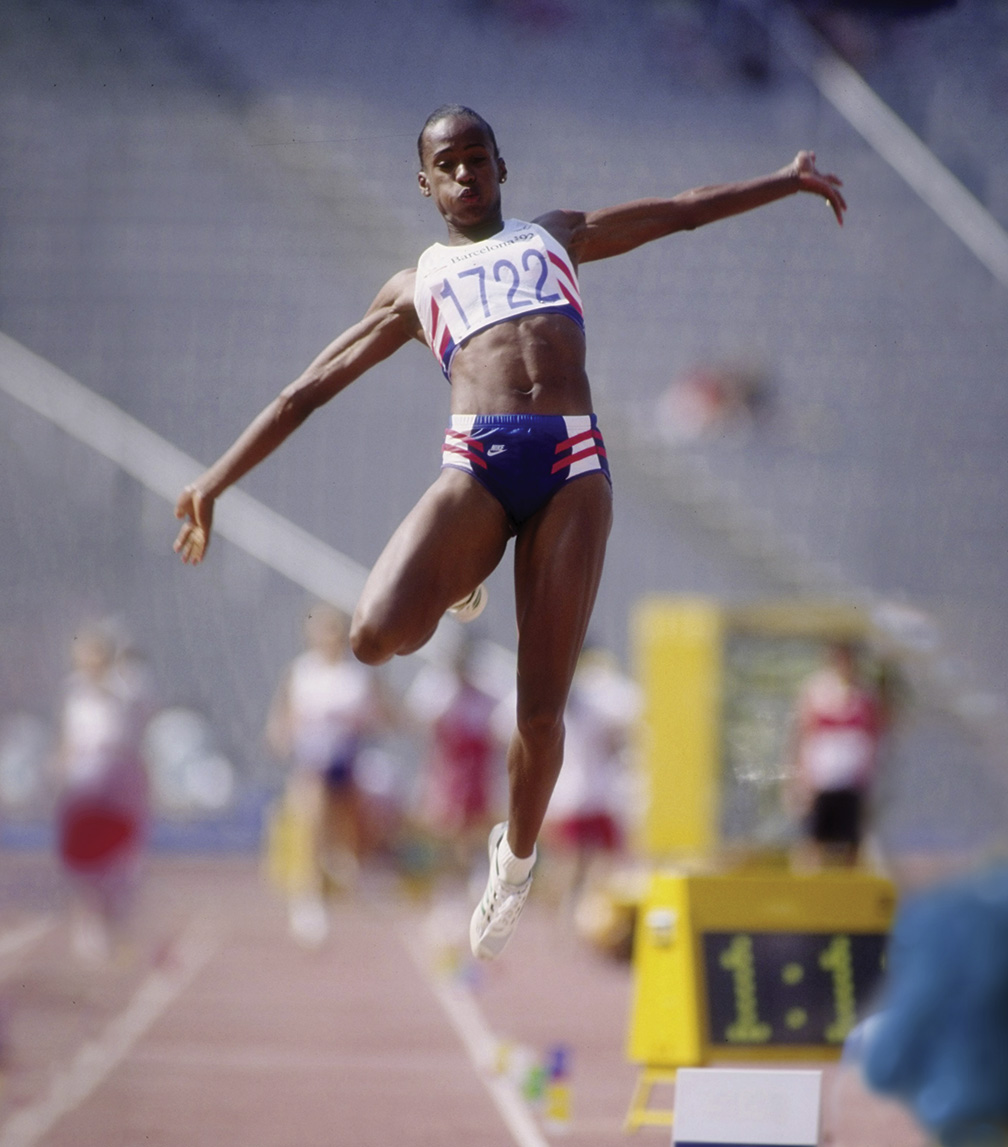
\includegraphics[width=1.0\linewidth]{chap13/13_0}
	% 加星号(*)表示不加编号
	\caption*{ \label{fig:13_0}}
\end{figure}

运动生物力学领域取得了长足的进步,但仍有更多领域有待探索。
本书介绍了测量、模型和计算工具如何帮助我们理解人类运动。
我们还展示了生物力学模型如何应用于机器人、跑道和外骨骼的设计。
生物力学使我们能够设计保护工人免受伤害的工厂,并制造出关节置换装置,使患有关节疾病的患者能够无痛行走。


这些成就改善了数百万人的生活,但我们也必须意识到现有知识和技术的局限性。
科技的新发展将使我们能够对人们的生活产生进一步的积极影响;
假肢功能的日益增强就是一个很好的例子。
知识的局限性更难克服。
克服这些局限性最重要的是,我们需要创造力,以及正如梭罗所说,勇于探索的勇气。


我想以我的一位合作者取得巨大成功的一次创造性飞跃作为本章的开篇。
接下来,我将描绘一幅我对生物力学领域的未来愿景——这幅愿景当然并不完整。
你的远见卓识将为这幅充满可能性的画布增添色彩和质感,在那里,你将拥有无限的空间去创造你的杰作。


\section{可穿戴技术}

凯特$\cdot$罗森布鲁斯在我的实验室工作时,在斯坦福医院遇到了一位男士,他因为一种叫做特发性震颤的疾病而无法给妻子写便条,也无法和朋友喝咖啡。
这是一种极其令人沮丧的疾病,但却非常常见。
五六十岁患上特发性震颤的人会因为手抖而无法进行日常生活活动。


这位患有特发性震颤的男子告诉凯特,他尝试过的药物并没有减轻他的手部震颤,而且副作用很大。
他唯一的选择就是手术,在脑部植入刺激电极。
这种疗法被称为深部脑刺激,已被证明对减轻震颤非常有效,但需要进行脑部手术。
脑部手术有严重并发症的风险。
这不是一个可以轻易做出的决定。


凯特知道,他的手颤抖很可能是由大脑特定区域的震荡神经活动引起的,其中包括丘脑腹侧中间核。
凯特找到一些文章,表明电刺激腕部正中神经会引发腹侧中间核内的神经活动。
她推断,刺激腕部的感觉神经或许能激发该脑区活动,从而无需手术即可减轻手部震颤。
作为一项实验,她决定尝试刺激几位自愿接受治疗的特发性震颤患者的正中神经。


这简直是​​一次盲目的尝试。
我们尚不清楚大脑震荡神经活动的确切原因,也不知道腕部电刺激是否会影响它。
但令我们(以及我们的参与者)欣喜的是,刺激正中神经后,他们的手部震颤显著减少。
这些初步数据激励着我们继续前进。
我们继续实验并学习这项新技术。
例如,当以与震颤相同的频率刺激正中神经时,我们发现效果最佳。
凯特与塞雷娜$\cdot$黄(Serena Wong)等人合作,打造了一款可穿戴运动传感器和神经刺激器,其外形类似腕表,可以记录患者手部震颤的频率,并以震颤频率刺激腕部神经。
令人欣慰的是,许多使用该设备的人的手部震颤显著减少\cite{lin2018noninvasive}。
他们恢复了写便条、喝咖啡以及进行其他用握手无法进行的活动的能力(图~\ref{fig:13_1})。


\begin{figure}[!htb]
	\centering
	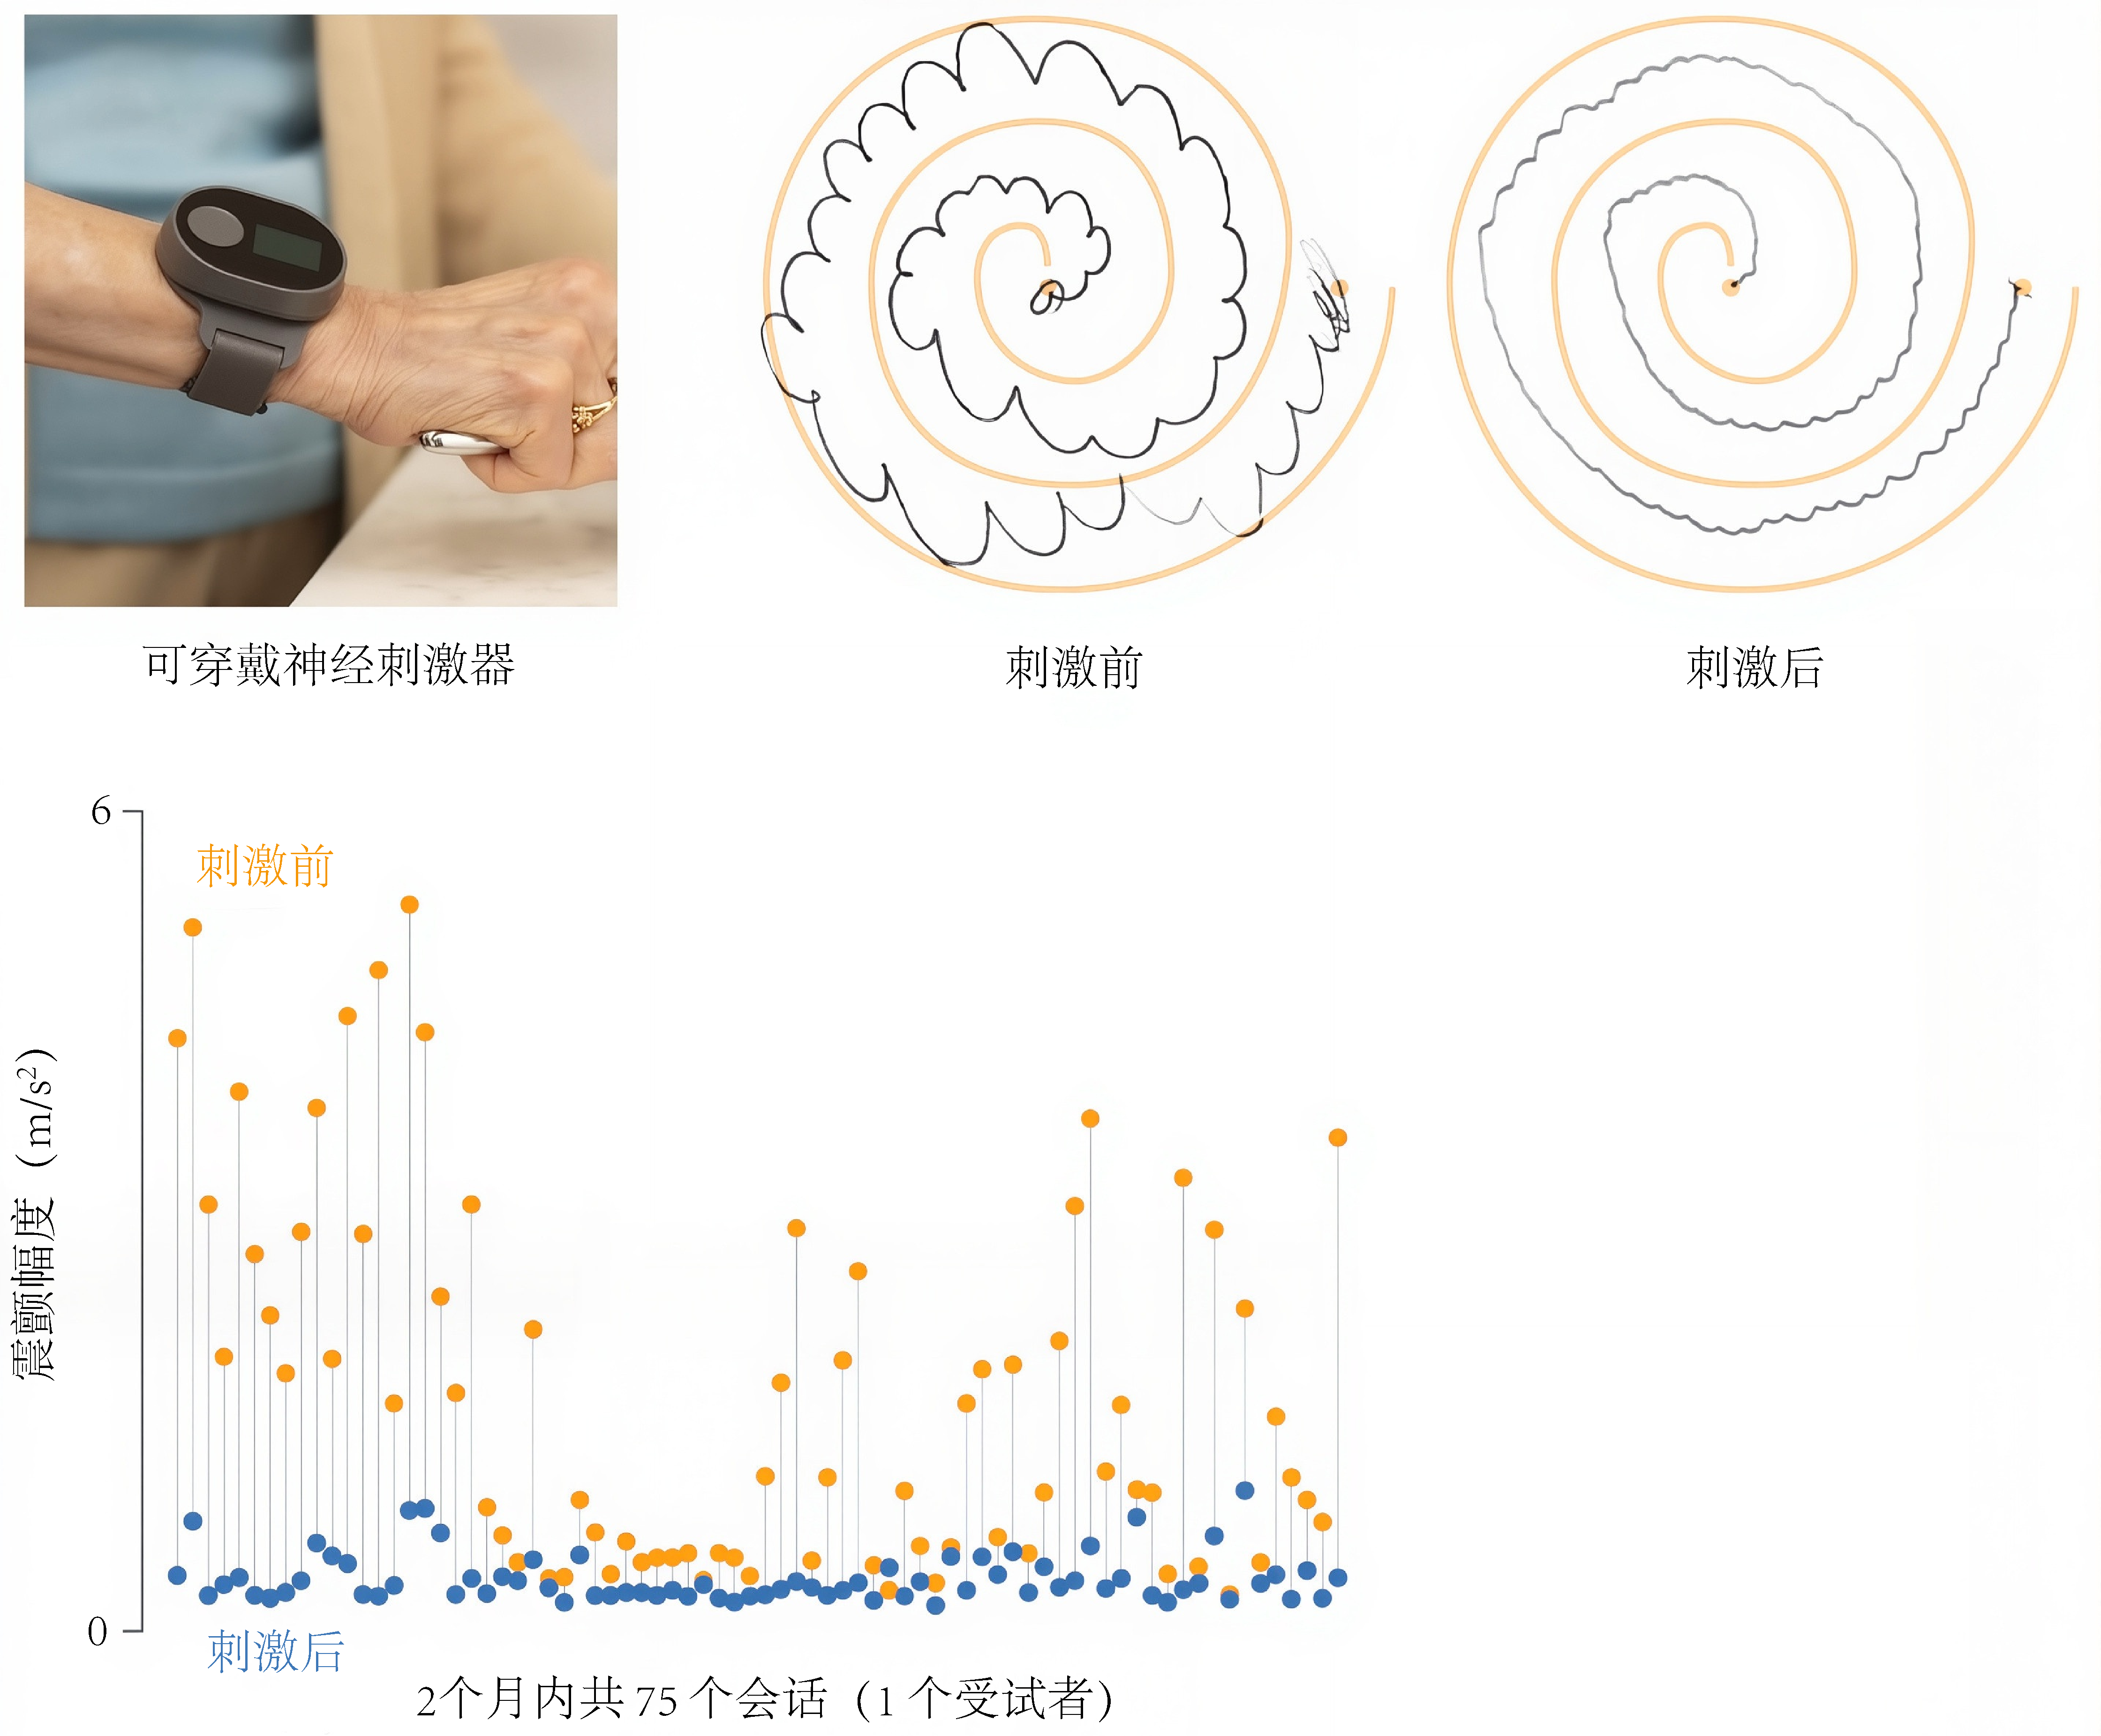
\includegraphics[width=1.0\linewidth]{chap13/13_1}
	\caption{可穿戴运动传感器和神经刺激器可减少手部震颤。
		Cala Health 的一款可穿戴刺激器(左上)显著减少了手部震颤(下图)。
		一位患者在接受 40 分钟神经刺激治疗后,螺旋画法显著改善(右上)。
		Cala Health, Inc. 是一家斯坦福大学衍生公司,由 Kate Rosenbluth、Serena Wong 和 Scott Delp 共同创立。 \label{fig:13_1}}
\end{figure}


这种新疗法无需药物和手术即可减轻手部震颤。
凯特的创造力和小型惯性测量单元使这项技术成为可能,这些单元可以记录患者的手部运动,使我们能够确定个性化的刺激模式。
神经刺激的效果,以及饮用咖啡或酒精(这些因素会影响手部震颤的程度)和其他因素的影响,可以在患者日常生活中持续数月进行监测。
未来,我们设想成千上万的患者佩戴神经刺激器,记录他们的手部运动并监测治疗效果,从而优化每位患者的功能。


小规模运动传感技术为推进治疗和研究提供了更多机遇。
目前,大多数生物力学实验都是在受控的实验室环境中使用本书所述的技术进行的。
但实验室测量存在严重的局限性。
例如,用于规划脑瘫儿童手术的步态分析通常依赖于在实验室这个陌生环境中仅测量几步的步数,这可能无法代表儿童在日常生活中的能力。
既然我们能够测量实验室外的运动,就可以开始使用在日常生活中几个月内测量的数千步步数来规划治疗方案。
我希望这能帮助我们做出更好的手术决策。


小型传感设备仍有很大改进空间。
目前可穿戴运动监测方法的精度不足以满足许多应用需求,尤其是在涉及运动模式受损人群的应用,准确区分功能性运动和症状性运动至关重要。
现实世界中,长时间佩戴传感器进行生物力学测量会产生大量噪声数据,我们需要新的方法来从这些海量数据集中获取洞见。
这为数据科学和生物力学领域的从业者提供了一个进行有意义互动的机会。


\section{随处可见的物理康复}

行走能力是独立生活的标志。
然而,中风、帕金森病和脑瘫等神经系统疾病和损伤严重限制了人们的活动能力。
骨关节炎等肌肉骨骼疾病会引发疼痛,并限制数百万人的行动能力。
总的来说,行动不便的后果广泛而严重。


康复对于改善行动障碍人士的生活至关重要。
多年来,我在康复诊所工作,深受人们渴望重拾能力的动力以及指导他们康复的治疗师的精湛技艺的鼓舞。
然而,目前的康复方法依赖于诊所内的评估和治疗。
物理治疗师和职业治疗师会评估患者并制定治疗方案,但他们缺乏衡量患者在诊所外活动能力的工具,也缺乏利用数百名类似患者数据来制定治疗方案的方法。
患者需要前往诊所就诊,加上高昂的治疗费用,限制了那些努力康复的患者能够获得的治疗数量。


我们必须开发工具,让患者无需前往诊所即可参与康复。
如果力量训练和活动训练可以在家进行,那么它们的开展频率就会更高。
移动传感器可以测量运动,但提供的信息并不完整。
我们还需要能够应用先进生物力学模型的软件,以精准量化行动障碍患者的运动。
通过优化这些工具,使其能够在智能手机上运行,​​并提供触觉、听觉和视觉反馈,我们可以将智能手机转变为运动测量系统和虚拟物理治疗师。
此外,机器学习方法可以从数千篇科学论文和描述数百万个体的数据(包括视频、临床记录和来自移动传感器的信号)中提取洞见,从而有可能以低成本提供有价值的指导。
对于我们这个领域来说,如何开发这些技术,使其能够为行动障碍患者带来切实的益处,而不是仅仅为了技术而开发技术,这将是一个挑战。


\subsection{大规模实验}

我做过的大多数研究都只有几十名参与者。
几年前,随着全球一些最大的公司开始对生物力学产生兴趣,数百万人开始携带配备运动传感器的智能手机,情况发生了改变。
我曾梦想能够进行大规模的实验。
随着全球大部分人口的手机都配备了加速度计,这个梦想或许可以成为现实。


我和我的合作伙伴与当地一家初创公司 Azumio Inc. 合作,收集并分析了来自 46 个国家/地区的 60 多万人的基于智能手机传感器的活动模式,这使得这次调查成为规模最大的体育活动调查,规模大约是前者的 1,000 倍。
我们发现,人群中活动最少和最活跃群体之间的不平等可以预测每个人群的肥胖患病率(图~\ref{fig:13_2})。
活动不平等用基尼系数计算,该公式也用于计算收入不平等。
基尼系数的范围从 0(每个人都获得平等的资源份额(完全平等))到 1(一个人获得所有资源)。
在活动不平等严重的国家,通常是因为大量女性相对不活跃;
在这些人群中,女性的预期寿命较低。
我们发现,在步行条件更好的城市,例如餐馆离住所和工作场所都在步行距离内的城市,活动不平等程度较低。
在这些适合步行的城市中,女性的体育活动增幅最大。
这些发现表明,城市规划和公共卫生政策应侧重于增加那些活动量最少的人群的活动量。
我建议生物力学家参与城市和社区规划,将体育锻炼融入日常生活。
这将对数百万人的健康产生巨大的积极影响。


\begin{figure}[!htb]
	\centering
	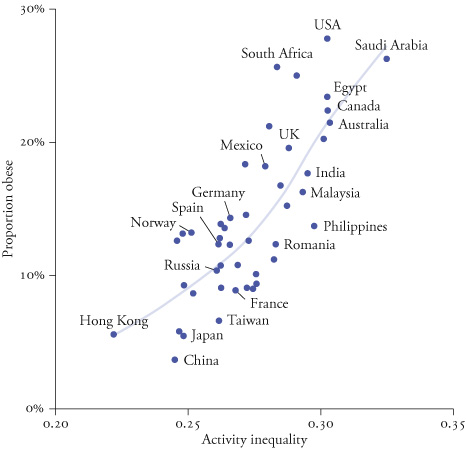
\includegraphics[width=0.75\linewidth]{chap13/13_2}
	\caption{活动不平等预测肥胖。
		活动不平等程度最高的五个国家/地区的个人肥胖可能性比活动不平等程度最低的五个国家/地区的个人高出196\% \cite{althoff2017large}。 \label{fig:13_2}}
\end{figure}


预计到2025年,全球移动医疗市场规模将增长至5000亿美元\cite{dwivedi2025digital}。
智能手机应用程序和可穿戴设备可用于监测各种健康行为,例如体力活动、步行速度、久坐时间、心率和睡眠。
分析可穿戴传感器和应用程序生成的数据,有可能改变我们研究人类行为以及干预改善健康的方式。
这些数据比传统研究收集的数据大得多,而且获取成本低廉。
由于数据是自动收集的,它们可以揭示自然环境中的行为,并惠及通常不参与研究的个体。


诸如体力活动\cite{world2010global}和久坐行为\cite{biswas2015sedentary}等可改变的行为对健康有着显著的影响,但在现代可穿戴传感器出现之前,用于大规模研究这些行为的工具一直有限。
来自应用程序和可穿戴设备的海量数据可以帮助我们发现促使健康行为的环境、社会和个人因素,并找到改善健康的新方法。


移动应用程序、可穿戴设备及其收集的海量数据具有变革性的潜力。
然而,有效分析这些数据需要生物力学、数据科学和公共卫生方面的专业知识。
很少有研究人员在这些领域接受过交叉培训,这使得跨学科的合作与沟通变得困难。
我努力积累数据科学和公共卫生方面的经验,以便能够与这些领域的研究人员交流,并指导那些想要跨越学科界限的学生。
这是一个你可以产生巨大影响的领域,我鼓励你深入研究。


大规模研究需要数据和先进的工具才能从中获得洞见。
遗憾的是,大多数研究实验室不愿共享其数据或工具。
一些公司维护着记录数百万个体活动的数据库,但这些数据库很少与研究人员共享进行分析。
生物力学的未来——乃至数百万个体的健康——要求我们开放这些数据,并开发从这些丰富的数据集中获取洞见的方法。


\section{现代统计学和机器学习}

几乎所有生物医学研究的结论都基于使用参数检验(例如学生 $t$ 检验)的假设检验。
然而,当前数据激增给包括生物力学在内的许多生物医学学科带来了新的挑战。
表征人体运动的数据具有高维性、异构性,并且随着可穿戴传感技术的发展而不断增长。
传统的统计方法限制了我们从这些数据中获得的洞察力。
新的统计方法将改变生物力学,就像它们在自动驾驶、图像识别和自动癌症检测领域所做的那样。


释放大数据集潜能的一种流行方法是机器学习。
Eni Halilaj 搜索了使用机器学习研究运动生物力学的研究论文,发现该领域的出版物数量正在快速增长(图~\ref{fig:13_3})。
随着越来越多的人参与生物力学和机器学习之间的协作和交叉训练,我预计这种趋势将会持续下去。


\begin{figure}[!htb]
	\centering
	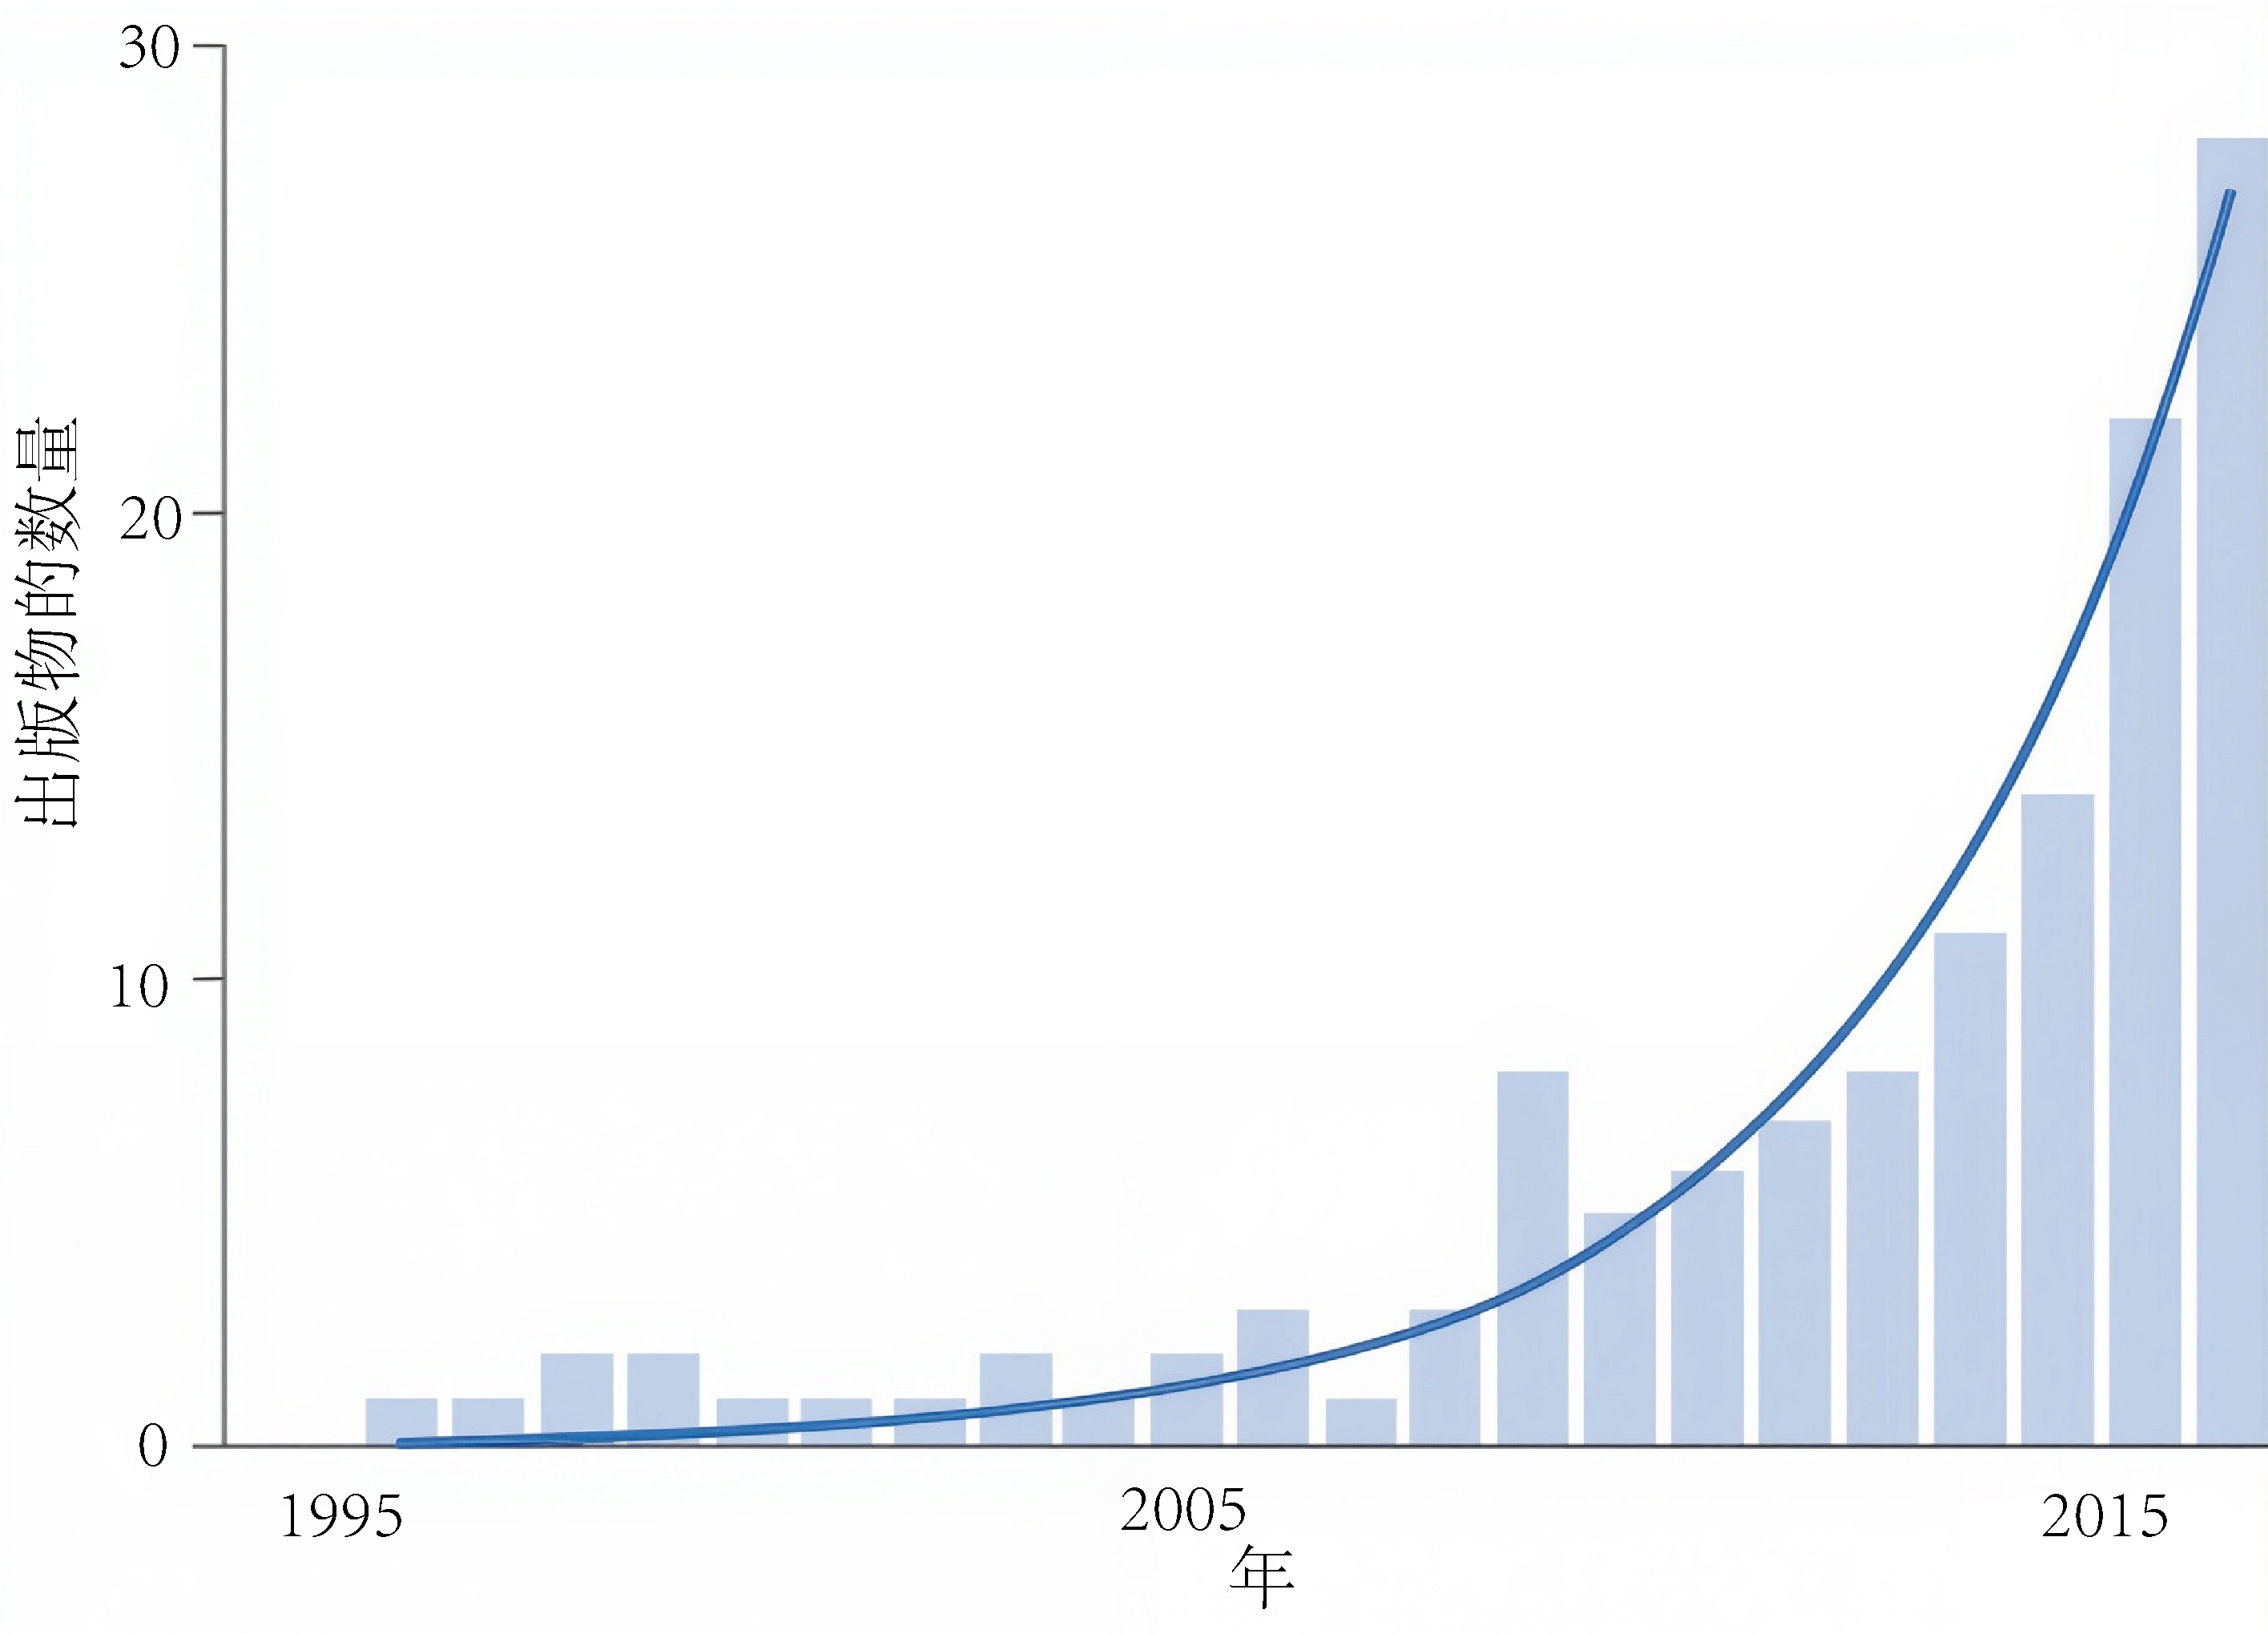
\includegraphics[width=0.75\linewidth]{chap13/13_3}
	\caption{近年来,数据科学方法在人体运动生物力学研究中的应用显著增加\cite{halilaj2018machine}。 \label{fig:13_3}}
\end{figure}


Apoorva Rajagopal 及其同事的研究说明了现代统计方法与生物力学建模相结合的影响。
Apoorva 的研究检查了马蹄足步态(用脚尖行走)的手术矫正,马蹄足步态是脑瘫儿童最常见的步态异常之一。
她想知道我们是否可以通过估计步态中的腓肠肌长度来确定哪些肢体的踝关节运动学可能在腓肠肌延长手术后得到改善(图~\ref{fig:13_4})。
她分析了 891 个接受手术的肢体的步态数据,并根据术前和术后踝关节运动学对结果进行分类。
接受腓肠肌延长手术的腓肠肌较短的肢体(“病例”肢体)比腓肠肌不短但仍接受延长手术的肢体(“过度治疗”肢体)更有可能获得良好的手术结果。
差异令人震惊:71\%的病例肢体在后续步态评估中取得了良好的结果,而过度治疗的肢体只有33\%取得了良好的结果(图~\ref{fig:13_5})。
她的研究结果表明,应该使用腓肠肌长度的估计值来判断哪些患者适合手术。

\begin{figure}[!htb]
	\centering
	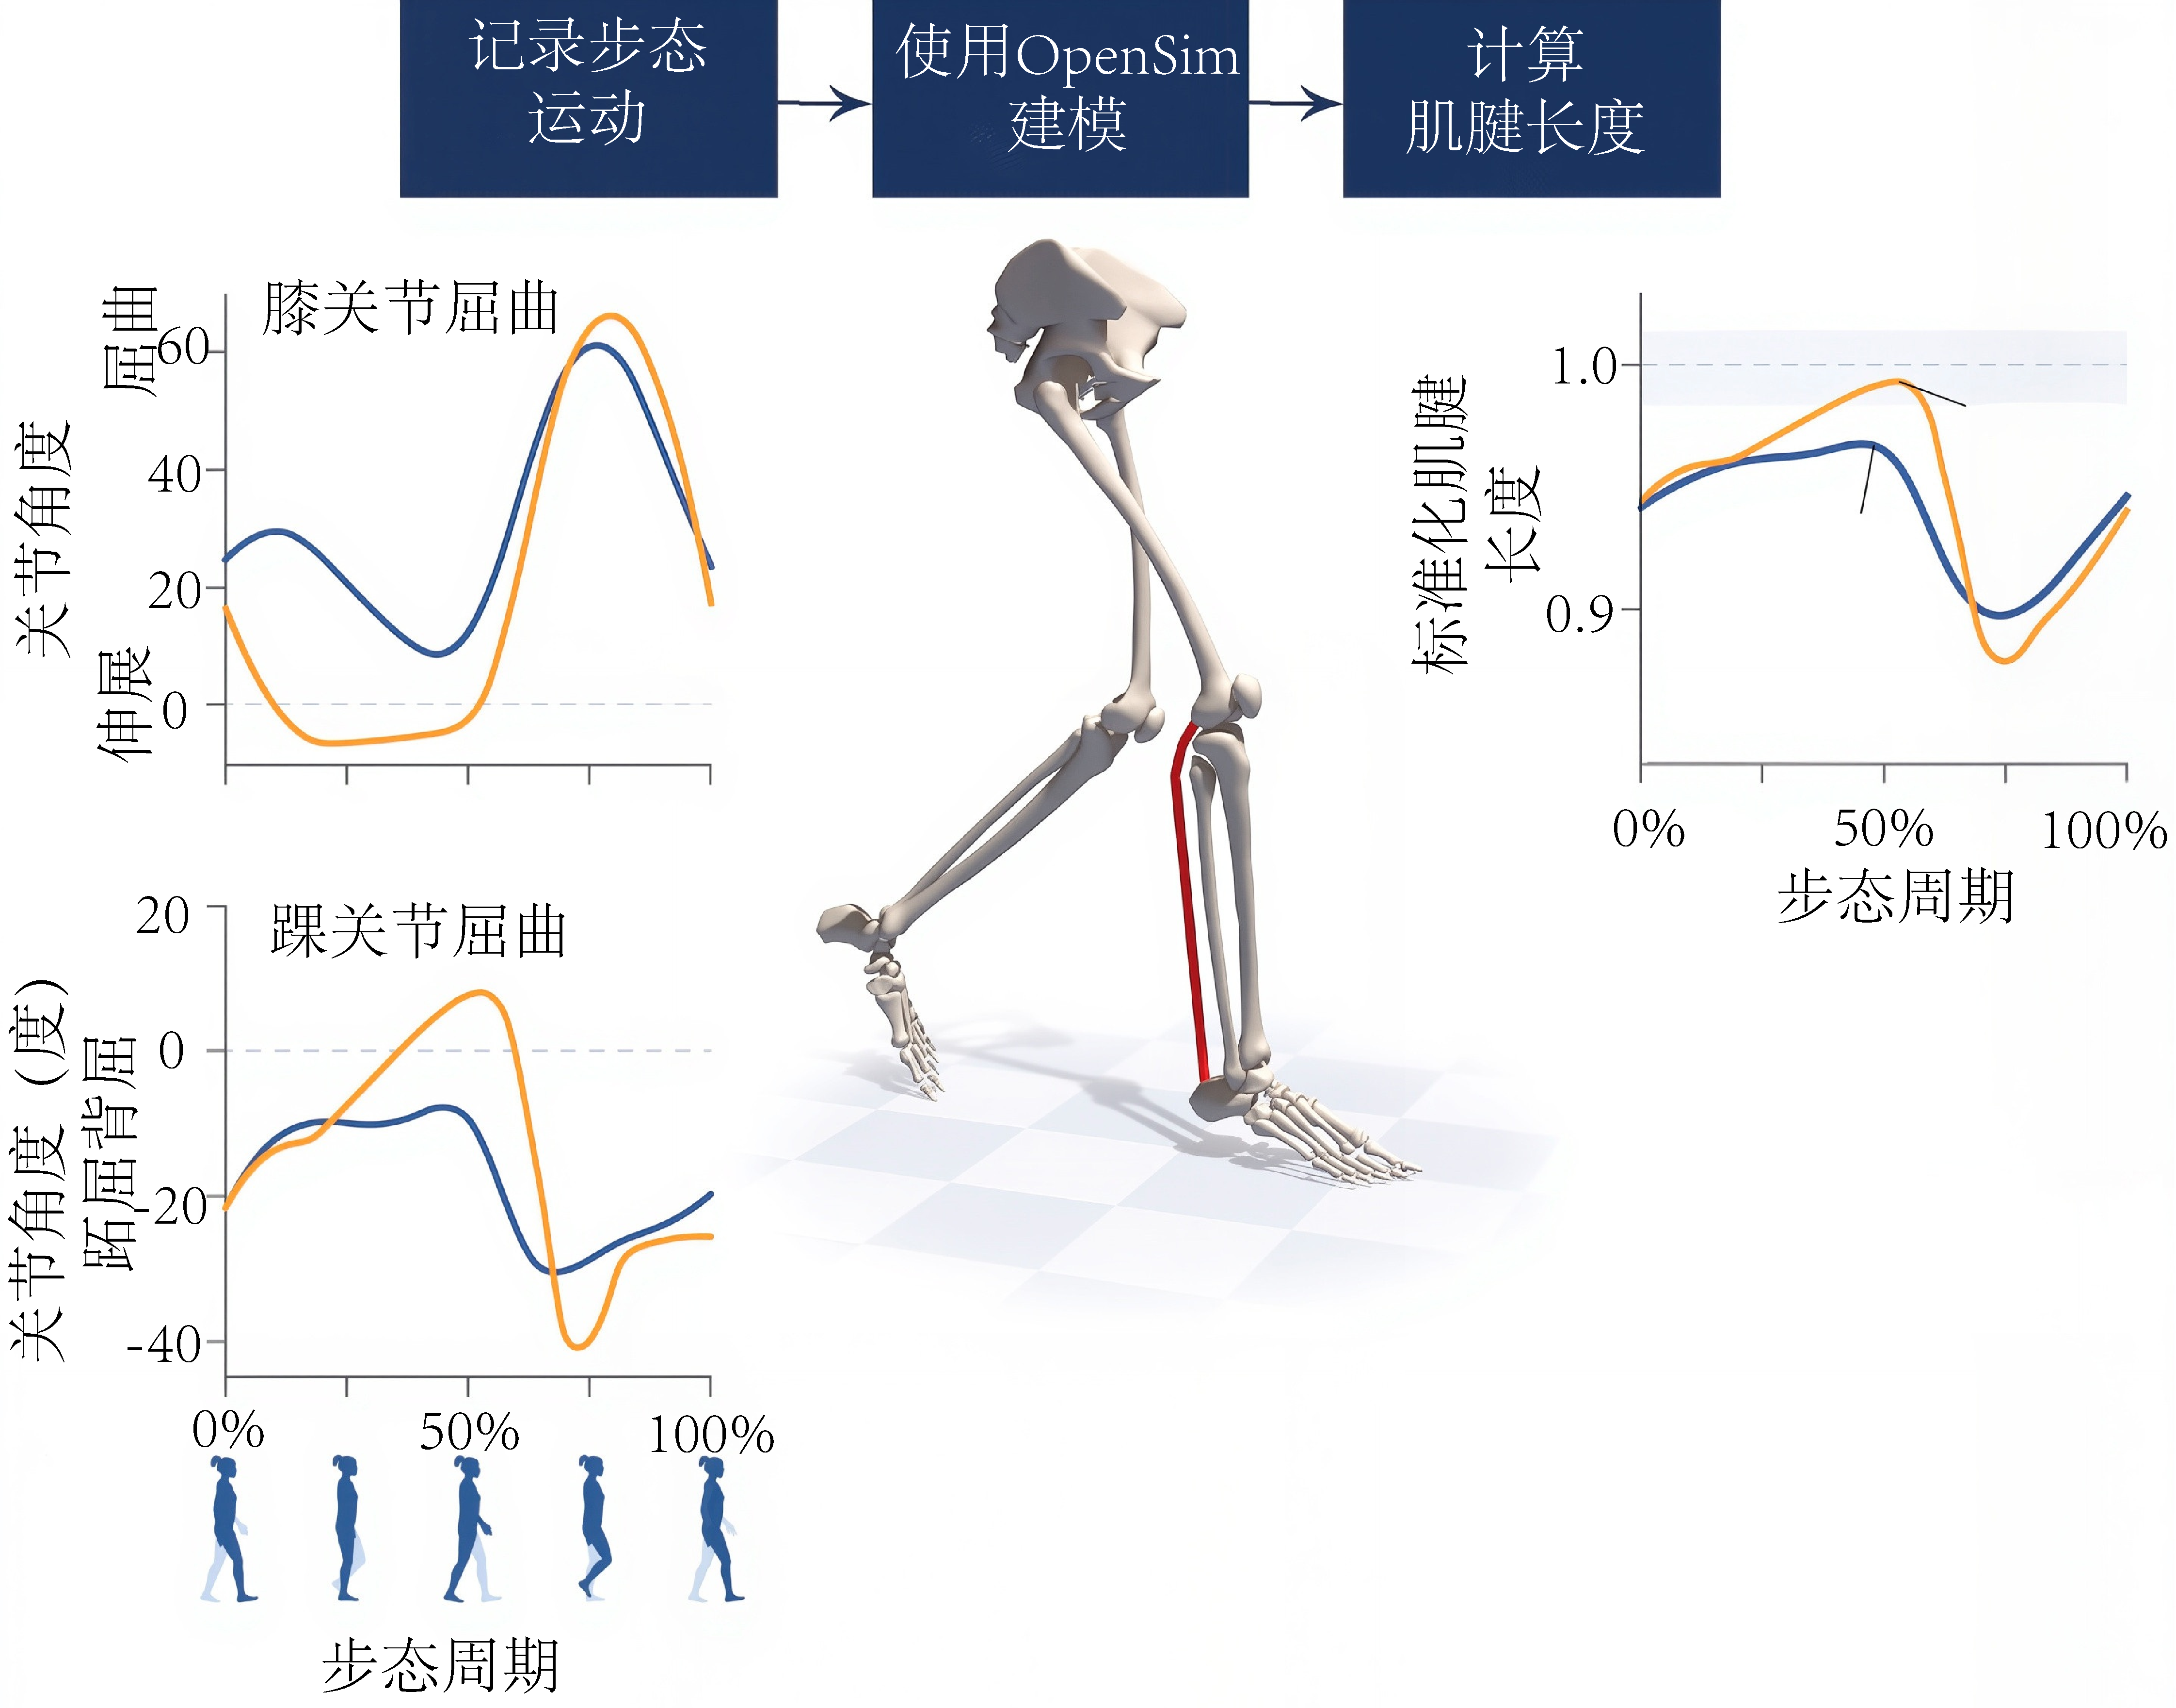
\includegraphics[width=1.0\linewidth]{chap13/13_4}
	\caption{腓肠肌长度估算方法。
		OpenSim 模型重现了运动捕捉记录的运动(左图),然后计算了腓肠肌内侧肌腱长度(右图)。
		这些长度被标准化为根据典型步态计算的平均峰值长度。
		峰值长度至少比典型平均值低 2 个标准差(即低于右侧面板中阴影带的长度)的肢体被归类为腓肠肌“短”。
		受试者 1(蓝线)的腓肠肌峰值长度较短,而受试者 2(橙线)的腓肠肌峰值长度较短\cite{rajagopal2020pre}。 \label{fig:13_4}}
\end{figure}


\begin{figure}[!htb]
	\centering
	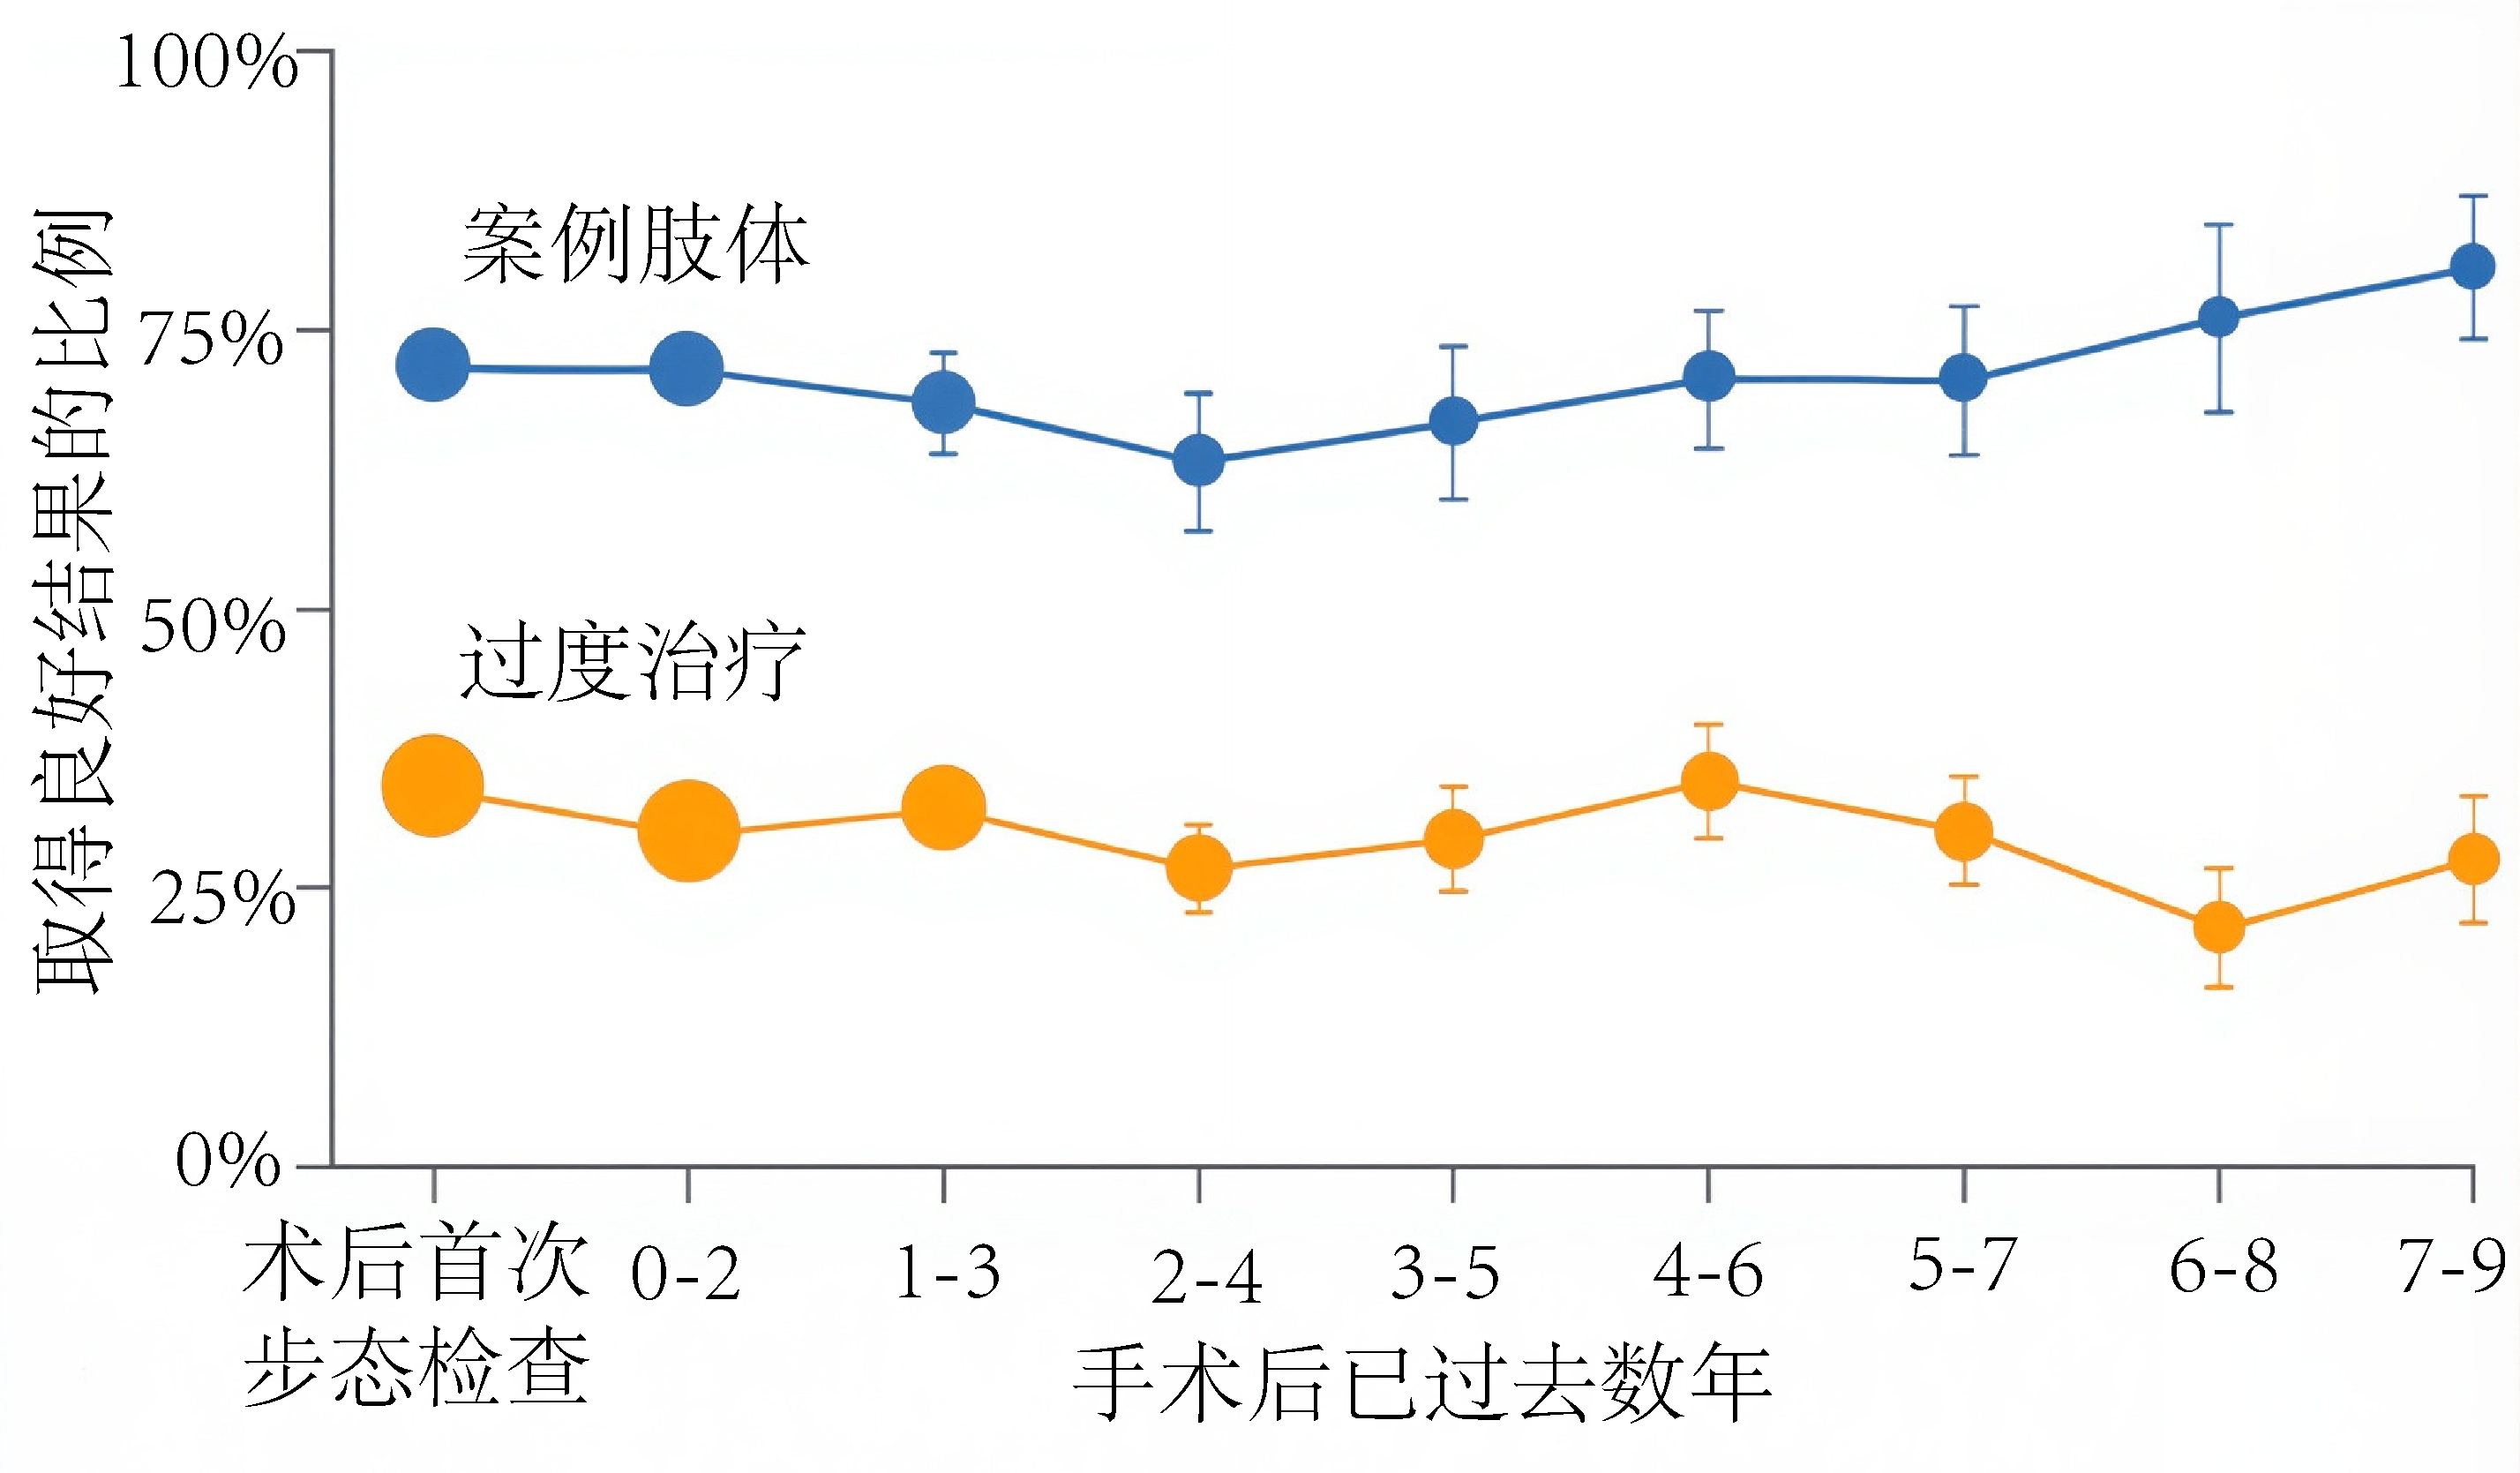
\includegraphics[width=0.7\linewidth]{chap13/13_5}
	\caption{腓肠肌延长手术后的长期疗效。
		病例组肢体接受了符合肌肉骨骼模型的手术,其疗效优于接受过度治疗的肢体。
		观察结果根据术后年数进行分箱,并计算每个分箱的良好疗效率。
		分箱在时间上重叠。
		误差线表示1个标准差;圆圈面积与观察次数成正比\cite{rajagopal2020pre}。 \label{fig:13_5}}
\end{figure}


\section{建立神经肌肉控制模型来预测运动}

模拟大脑如何协调运动是生物力学领域的一大挑战。
计算建模大多局限于重现观察到的运动,以研究无法测量的量,例如肌肉力量和关节负荷。
现代计算技术推动了预测模拟的发展,这种模拟无需事先收集实验数据即可生成运动模拟。
预测模拟使用优化来实现高级目标,例如最小化模型在步态过程中的能量消耗,同时遵循牛顿定律等物理约束和肌肉激活延迟等生理约束。
优化问题中的变量描述了如何协调模型的肌肉。
只要优化问题能够捕捉到真实运动的显著特征,解决方案就能生成一个模拟,该模拟代表自然界中观察到的运动。
预测模拟将使我们能够设计出更好的假肢和手术,从而最大限度地发挥个体的功能。


为了生成预测模拟,我们必须解决高维优化问题。
解决这些问题的一种策略是使用强化学习,它无需了解底层模型,也无需设计控制器的结构:优化器只需学习如何生成模型输入(在本例中是随时间变化的肌肉刺激),从而产生理想的输出。
Łukasz Kidziński\cite{learning2018learning}在过去两届神经信息处理系统大会期间举办了一场精彩的竞赛,超过一千名参赛者使用强化学习来解决运动控制中的经典问题。
例如,参赛者面临的挑战是开发控制器,使肌肉骨骼模型能够在不平坦的地形上奔跑。
结果令人惊叹!参赛者证明了强化学习技术可以合成行走和跑步等自然动作。
他们的优化器还发现了各种奇特的跳跃和跳跃步态。
该项目的成功得益于生物力学家和计算机科学家的合作,以及 OpenSim 等强大的开源软件和 CrowdAI 的强化学习环境。


直接配点法是解决生物力学中高维优化问题的另一种有效方法。
直接配点法将运动方程转换为代数约束方程,有效地同时计算所有时间帧。
解决优化问题极具挑战性,研究人员通常需要等待数天甚至数周才能获得优化结果。
直接配点法已被用于解决生物力学中的最优控制问题,其速度远快于传统方法,并将使预测模拟的用途更加广泛。
我确信直接配点法将对生物力学的未来产生巨大影响,并鼓励您进一步了解它。


\section{激励运动}

我们都知道,体育锻炼有益健康。
正如希波克拉底的名言:“行走是人类最好的良药。” 
然而,近一半的成年人未能获得足够的运动来维持健康,这种缺乏运动的状况正在给我们带来高昂的代价。
全球每年有500万人死于心脏病、中风和糖尿病等疾病,而其中许多疾病只需增加体育锻炼即可预防\cite{lee2017reducing}。
能够激励健康行为(尤其是像运动这样已被广泛接受且成本较低的行为)的技术,可以改善数百万人的健康,并减轻缺乏体育锻炼带来的经济负担。


智能手机和可穿戴传感器有潜力实现这一愿景,并彻底改变医疗保健。
我之前提到过,这些设备提供了大量关于身体活动的数据,智能手机能够与用户进行近乎持续的互动,从而激励健康行为。
然而,智能手机和其他设备并没有改善健康状况,有些甚至产生了相反的效果\cite{jakicic2016effect}。
显然,单靠技术能力不足以解决这个问题。
如果我们想让这些设备成为改善公共健康的积极工具,而不仅仅是收集信息,我们就必须了解人们如何与科技互动。
激励个人远比仅仅开发一个漂亮的新设备要复杂得多。


身体活动是一种强效且低成本的良药,但我们需要精准且引人入胜的工具来激励它。
行为心理学、人机交互理论和生物力学等不同学科的理念已在小范围内取得成功;然而,这些创新很少被融入移动健康应用中。
生物力学家必须与其他学科的专家合作,探索激励身体活动的新方法,以惠及全球数百万人,并解决神经系统残疾等亟需解决的领域。
我们的愿景是实现有效且价格合理的医疗保健,并在全球范围内推广。

\section{开放科学}

开放科学是推动我们领域发展的最佳途径。
作为一个群体,我们必须向所有人免费开放出版物、数据、模型和软件。
我们已经从健康个体以及患有各种运动障碍的个体中收集了海量高保真运动数据。
但这些数据隐藏在计算机硬盘中,无法供整个群体访问。
匿名化并发布这些数据将使前所未有的生物力学研究成为可能。
为了鼓励数据共享和开放科学,我和我的同事创建了一个用于共享生物力学数据、模型和软件的网站——\href{simtk.org}{simtk.org},该网站托管着超过 1000 个共享资源的项目。
本书中介绍的模型和数据均可在此网站上获取。
生物力学文化必须持续变革,使数据共享成为常态。


共享软件也能加速研究进程。
生物力学模拟正迅速普及,部分原因在于它是实验方法的有力补充,同时也因为现在已经有了成熟的软件工具。
正如我们在本书中所见,OpenSim 软件使用户能够构建生物力学模型、模拟肌肉骨骼动力学、预测新动作并传播新的计算工具。
Jeff Rankin、Jonas Rubenson 和 John Hutchinson(2016)使用 OpenSim 研究了鸵鸟(奔跑速度最快的双足动物)拥有惊人速度、敏捷性和效率的机制(图~\ref{fig:13_6})。
Taymaz Homayouni 及其同事\cite{homayouni2015modeling}使用 OpenSim 制作了新的可植入机制原型,以恢复手臂部分瘫痪患者的功能。
Matt DeMers、Jennifer Hicks 和我使用 OpenSim 比较了反射和准备性肌肉协同激活在预防踝关节损伤方面的有效性(图~\ref{fig:13_7}),这项研究如果通过实验进行会过于危险。
这些只是 OpenSim 软件支持的数百项研究中的一小部分,我很高兴看到 OpenSim 社区不断发展壮大。


\begin{figure}[!htb]
	\centering
	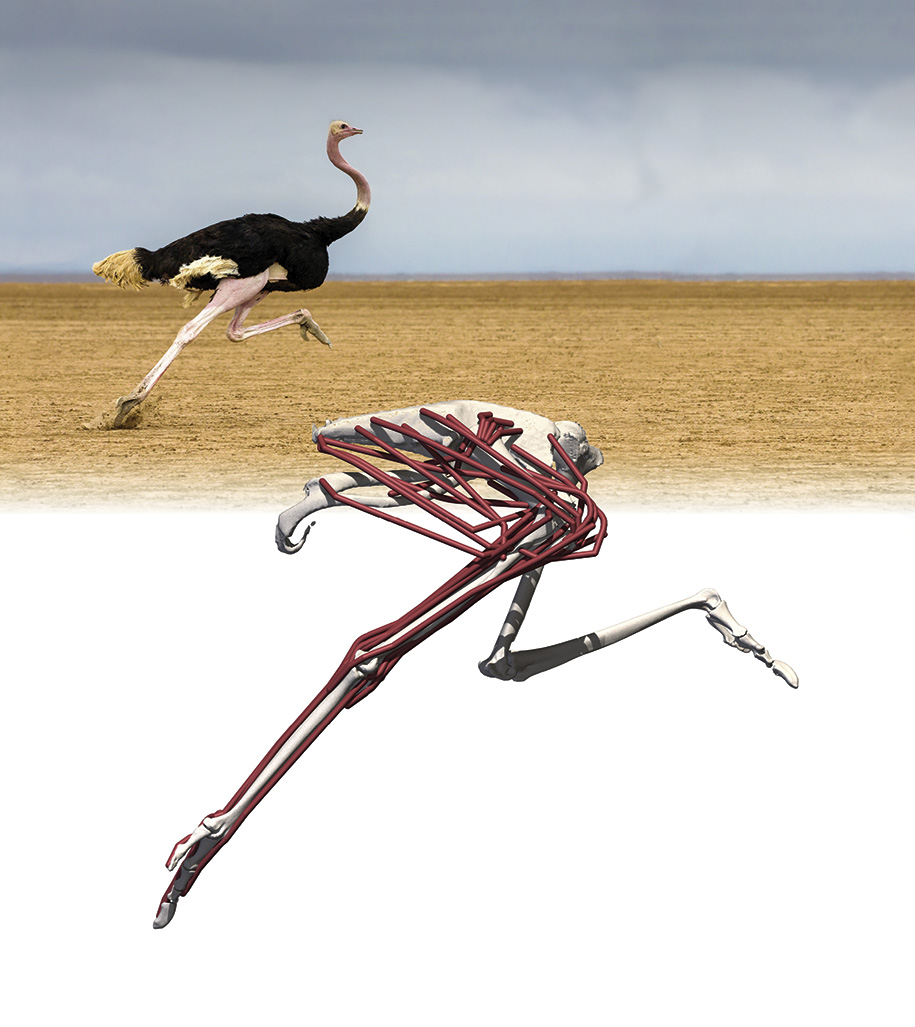
\includegraphics[width=0.9\linewidth]{chap13/13_6}
	\caption{鸵鸟的 OpenSim 模型,鸵鸟是地球上跑得最快的双足动物\cite{rankin2016inferring}。 \label{fig:13_6}}
\end{figure}


\begin{figure}[!htb]
	\centering
	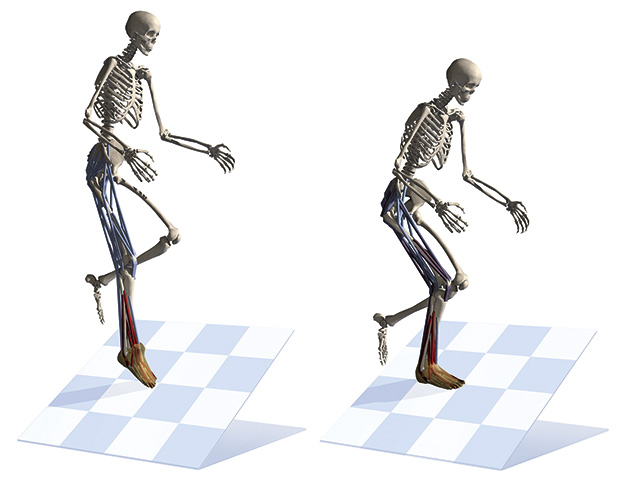
\includegraphics[width=1.0\linewidth]{chap13/13_7}
	\caption{用于研究踝关节损伤的斜坡落地模拟帧。OpenSim 模型来自 DeMers 等人\cite{demers2017preparatory}。 \label{fig:13_7}}
\end{figure}


除了开源软件之外,肌肉骨骼结构计算模型的开放获取也促进了广泛的研究。
例如,Sam Hamner 的跑步模拟模型(图~\ref{fig:12_4})、Miguel Christophy 的腰椎模型\cite{christophy2012musculoskeletal}以及 Kate Saul 的上肢模型(图~\ref{fig:10_6})已被成千上万的研究人员和学生使用。
持续推进开放科学的趋势将有助于研究日益复杂的问题,这些问题只有通过拥有不同专业知识的人员的共同努力才能解决。
OpenSim 项目提供了一个协作研究平台,支持一个多元化、全球化且不断扩张的社区,致力于解决生物力学领域最重要的问题(图~\ref{fig:13_8})。
我希望您能加入这个团队。


\begin{figure}[!htb]
	\centering
	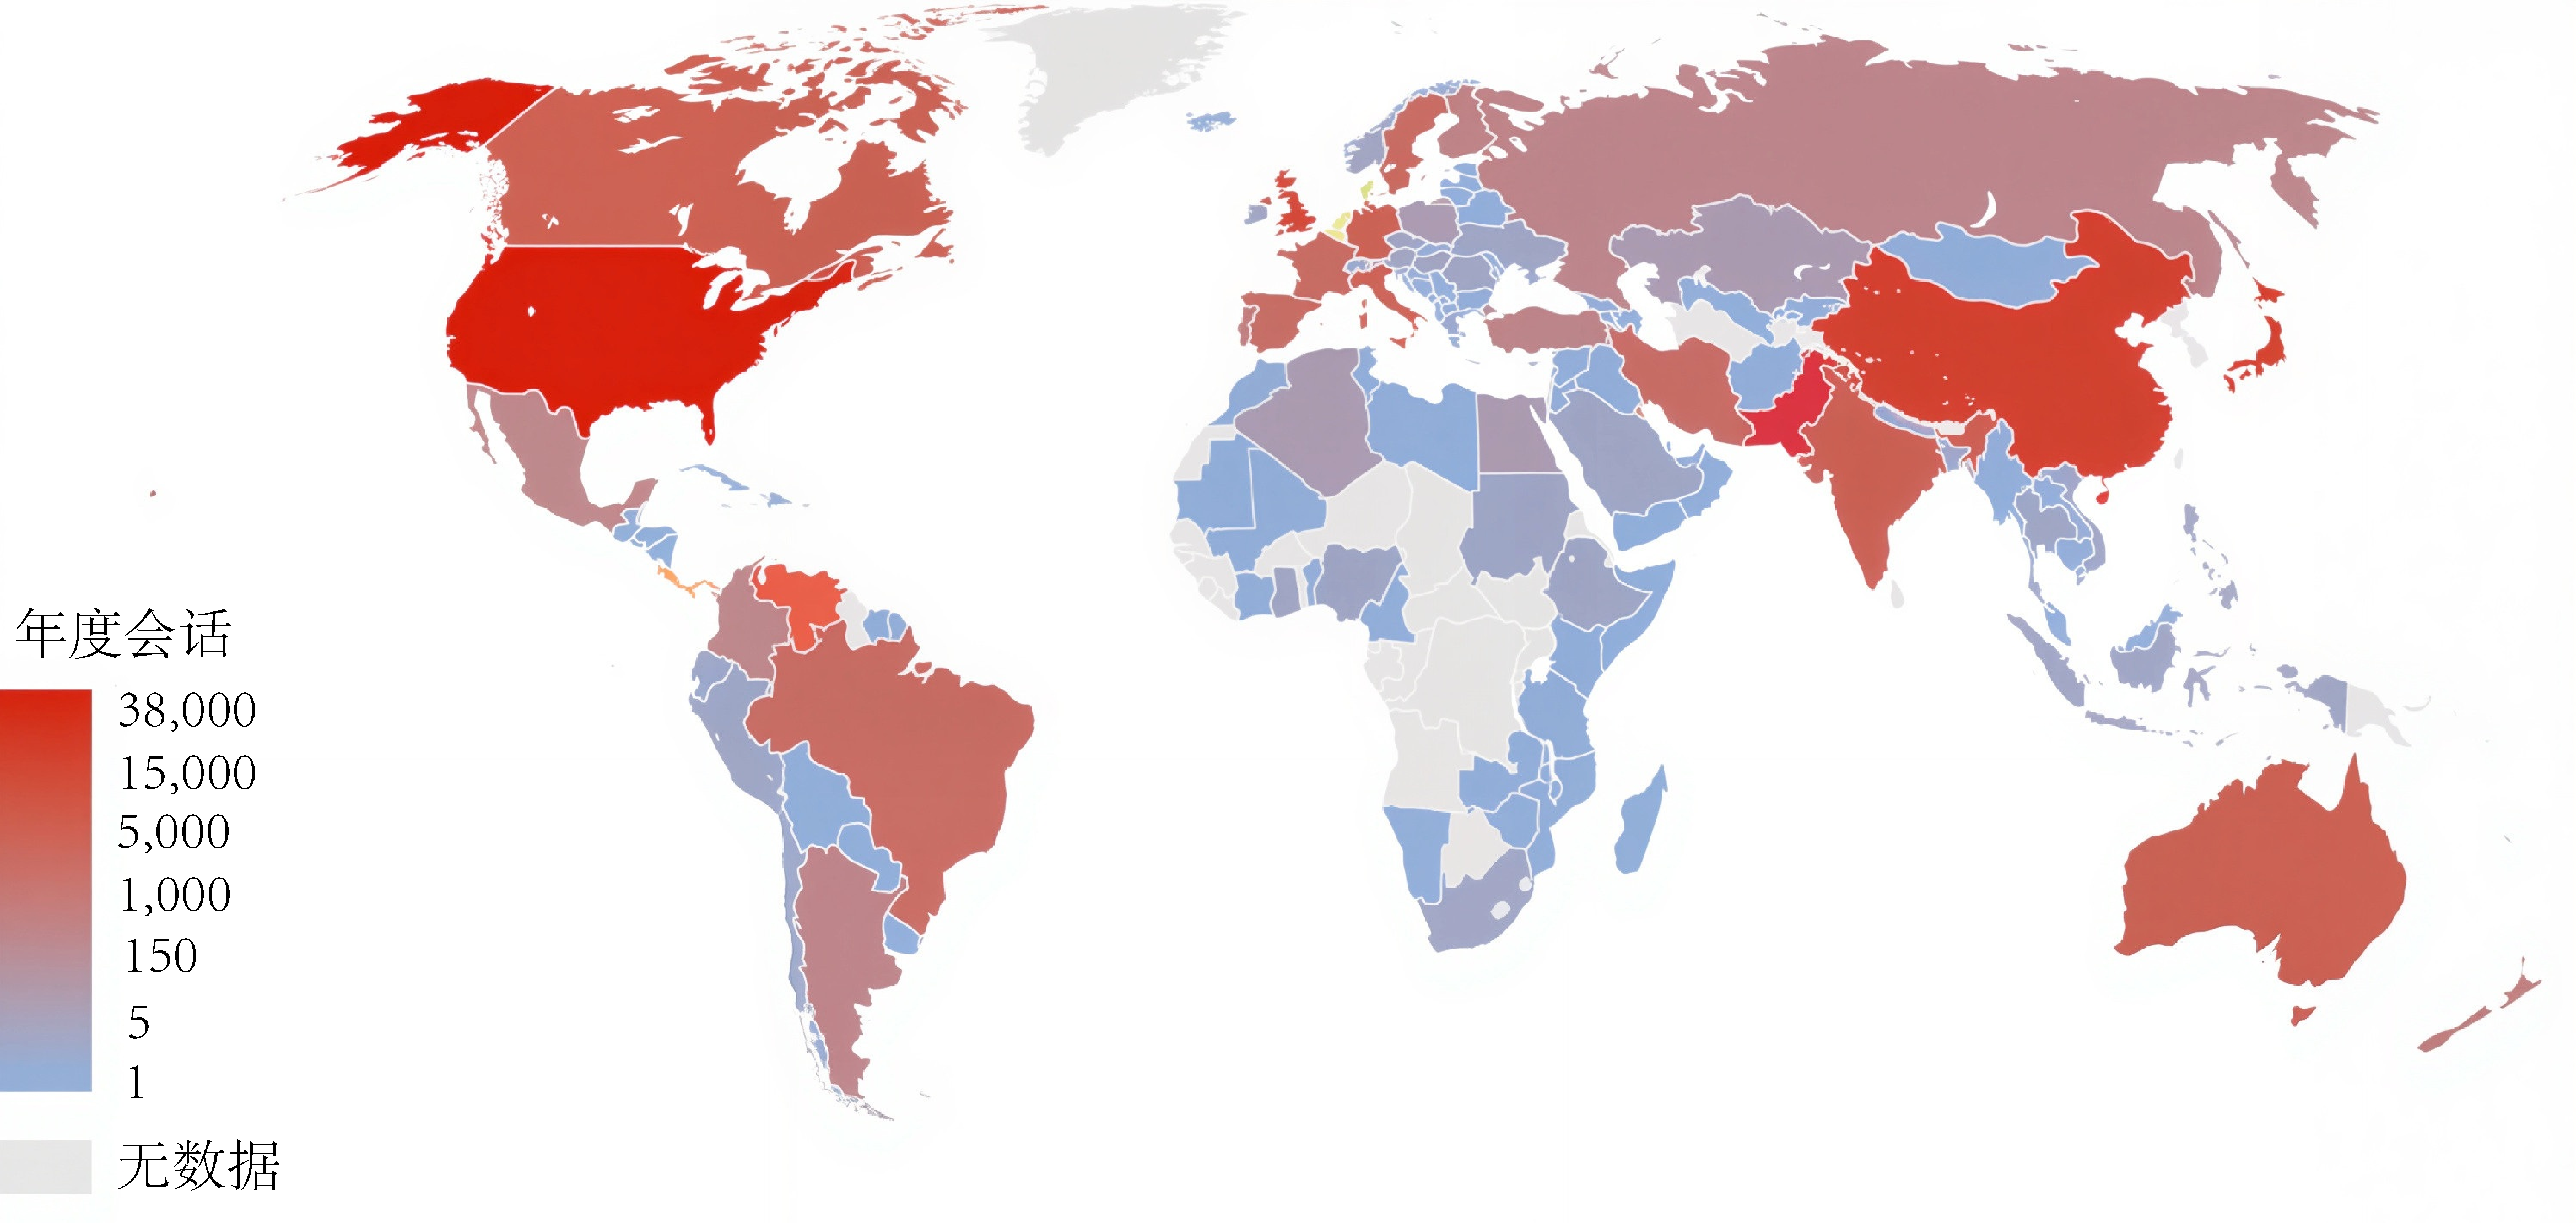
\includegraphics[width=1.0\linewidth]{chap13/13_8}
	\caption{最近一年内访问 OpenSim 文档的访客所在地。
		自 2012 年上线以来,OpenSim 文档 wiki 每年吸引来自世界各地的超过 25,000 名用户访问\cite{seth2018opensim}。 \label{fig:13_8}}
\end{figure}


\section{接过接力棒}

我希望本书能加深您对人体运动的优雅和复杂性的理解。
即使我们涵盖的有限内容,也是数千人数百年来共同研究的结晶。
这是一个令人惊叹的团队合作。
正如沃尔特$\cdot$惠特曼所写:“精彩的演出仍在继续,而您或许可以贡献一首诗。” 
的确,您通过本书所学到的原理,为您参与该领域奠定了基础。
您可以用全新的视角阅读有关跑鞋和机器人的新闻文章和期刊论文。
您可以参加研讨会或会议,或者只是和朋友聊聊我们的运动方式。
只要稍加创意,再加一点努力,您就可以通过生物力学为世界做出有意义的贡献。
让我们继续前进!









